\documentclass[11pt,letterpaper]{article}
\usepackage[utf8]{inputenc}

\usepackage[margin=1in]{geometry}
\usepackage{graphicx}
\newcommand{\floor}[1]{\lfloor #1 \rfloor}
\usepackage[normalem]{ulem}
\useunder{\uline}{\ul}{}
\usepackage{multicol}
\usepackage{textcomp}
\usepackage{enumerate}
\usepackage{enumitem}
\usepackage{float}
\usepackage{longtable}
\usepackage{hyperref}
\usepackage{commath}
\usepackage{amssymb}
\title{Práctica 1. Cambio de color de la linea de comandos.}
\usepackage{listings}
\usepackage{color}
\usepackage{graphicx}
 
\definecolor{codegreen}{rgb}{0,0.5,0}
\definecolor{codegray}{rgb}{0.5,0.5,0.5}
\definecolor{codepurple}{rgb}{0.58,0,0.82}
\definecolor{backcolour}{rgb}{0.95,0.95,0.92}
 
\lstdefinestyle{mystyle}{
    backgroundcolor=\color{backcolour},   
    commentstyle=\color{codegreen},
    keywordstyle=\color{magenta},
    numberstyle=\tiny\color{codegray},
    stringstyle=\color{codepurple},
    basicstyle=\footnotesize,
    breakatwhitespace=false,         
    breaklines=true,                 
    captionpos=b,                    
    keepspaces=true,                 
    numbers=left,                    
    numbersep=5pt,                  
    showspaces=false,                
    showstringspaces=false,
    showtabs=false,                  
    tabsize=2
}

 
\lstset{
style=mystyle,
literate={á}{{\'a}}1
        {ã}{{\~a}}1
        {é}{{\'e}}1
        {ó}{{\'o}}1
        {í}{{\'i}}1
        {ñ}{{\~n}}1
        {¡}{{!`}}1
        {¿}{{?`}}1
        {ú}{{\'u}}1
        {Í}{{\'I}}1
        {Ó}{{\'O}}1
}

\usepackage{enumerate}
\usepackage{enumitem}

\usepackage{longtable}
\usepackage{hyperref}
\usepackage{commath}

\begin{document}
\title{\vspace{-1.5cm}
	Práctica 3\\
    \large Universidad Nacional Autónoma de México\\
    Facultad de Ciencias\\
    Administración de Sistemas Unix/Linux\\
}
\author{
    Miguel Torres Eric Giovanni\\
    \url{https://github.com/EricGiovanni} \and
    Esquivel Guzmán Karla Adriana \\
    \url{https://github.com/karlycaramelo} \and
    Lezama Hernández María Ximena\\
    \url{https://github.com/LezamaXi} \\ \and
    Vazquez Cruz Gonzalo\\
    \url{https://github.com/truerandom} \\
    }
\date{1 de Marzo 2019}
\maketitle


\section{Introducción}

Arch Linux es una distribución GNU/Linux de propósito general. La instalación por defecto deja un sistema de base mínima, que el usuario configurará posteriormente agregando lo que necesite. Arch Linux define simplicidad como sin adiciones o modificaciones innecesarias. 

Los archivos de configuración de Arch proporcionados por los desarrolladores contienen cambios limitados relativos a cuestiones específicas de la distribución, como el ajuste de las rutas de los archivos del sistema. No añade características de automatización, tales como activar un servicio simplemente porque se ha instalado el paquete. 

Instalar Arch Linux es algo comparable a construir tu propia casa. Tienes que excavar los cimientos, levantar las paredes, construir los techos, instalar la fontanería y la electricidad... Y luego todo lo que falta. En pocas palabras, Arch Linux no es comparable a cualquier otra distro, que instalas y está lista para funcionar con su escritorio y su lista de software base.
 \begin{figure}[H]
        \centering
        
\includegraphics[width=0.8\textwidth]{img/1.png}
        \label{img:Imagen 1}
\end{figure}

\section{Objetivo}

El objetivo de esta practica es instalar Arch Linux en una maquina virtual, haciendo todo a mano, y montando lo necesario sin utilizar el script \textit{arch-chroot}.

Arch Linux es una distribución de propósito general x86-64 que es popular entre los entusiastas del bricolaje y los usuarios incondicionales de Linux. La instalación predeterminada cubre solo un sistema base mínimo y espera que el usuario final lo configure y lo use. Basado en KISS, \textit{¡manténlo simple, estúpido!} En principio, Arch Linux se centra en la elegancia, corrección de código, sistema minimalista y simplicidad.

Además, es uno de los sistemas operativos más populares para aprender Linux desde cero. 

\section{Instalación}

Antes de instalar Arch Linux desde un USB, hay que asegurarnos de tener los siguientes requisitos:
\begin{itemize}
    \item Una máquina compatible x86\_64 (es decir, 64 bit)
    \item Mínimo 512 MB de RAM (recomendado 2 GB)
    \item Al menos 1 GB de espacio libre en disco (se recomiendan 20 GB para uso básico)
    \item Una conexión a internet activa
    \item Un dispositivo USB con un mínimo de 2 GB de capacidad de almacenamiento
\end{itemize}

Los prerrequisitos son : descargar la imagen del disco, se puede descargar el ISO desde el sitio web oficial de \textbf{Arch Linux}, y tenerla descargada para su intalación. 

Así como crear previamente una maquina virtual con los requisitos necesarios para instalar \textbf{Arch}, en esta practica usamos \textit{Virtual Box} para crear la maquina virtual.

Una vez ya iniciado saldrá la siguiente pantalla, y selecciona Boot Arch Linux (x86\_64). Después de varias comprobaciones, Arch Linux iniciará la solicitud de inicio de sesión con el usuario root.

 \begin{figure}[H]
        \centering
        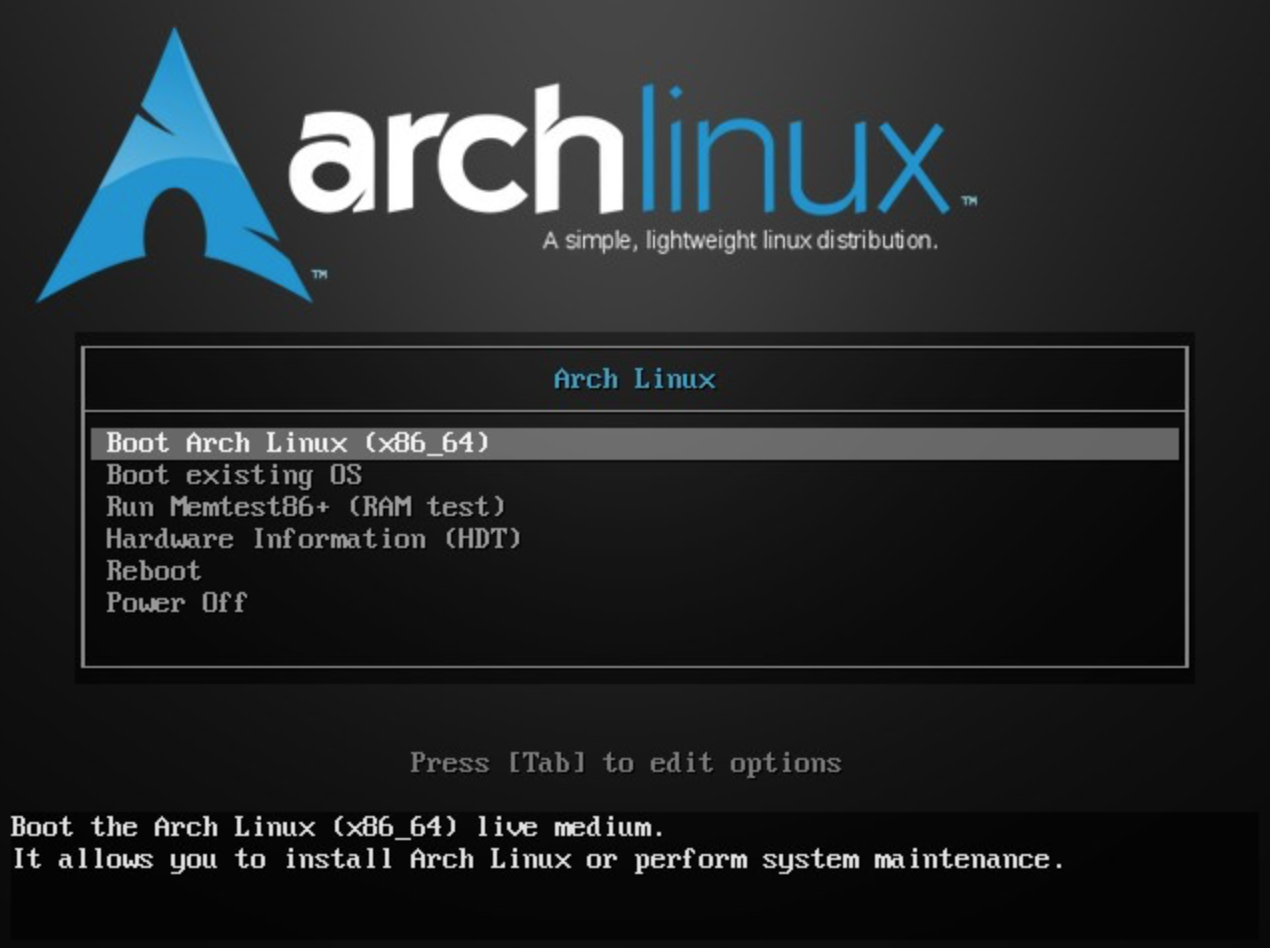
\includegraphics[width=0.8\textwidth]{img/2.png}
        \label{img:Imagen 1}
\end{figure}

Los próximos pasos incluyen la partición del disco, la creación del sistema de archivos y su montaje.

\subsection{Configuración}
El primer paso incluye la partición de tu disco duro. Una sola partición raíz es la más simple en la que crearemos una partición root (/). Nosotros crearemos 3:
\begin{itemize}
    \item / $\rightarrow$ sda1
    \item swap $\rightarrow$ sda2
    \item /home $\rightarrow$ sda3
\end{itemize}
  Para crear una partición. Se utiliza el comando:
  \begin{center}
      fdisk /dev/sda
  \end{center}
  Una vez ejecutado el comando, se escribe "\textit{n}" para una nueva partición. Escribe "\textit{p}" para una partición primaria y selecciona el número de partición.
  
  El primer sector se selecciona automáticamente y solo necesitas presionar \textit{Enter}. Para el último sector, escribe el tamaño que deseas asignar a esta partición.
 
  \begin{figure}[H]
        \centering
        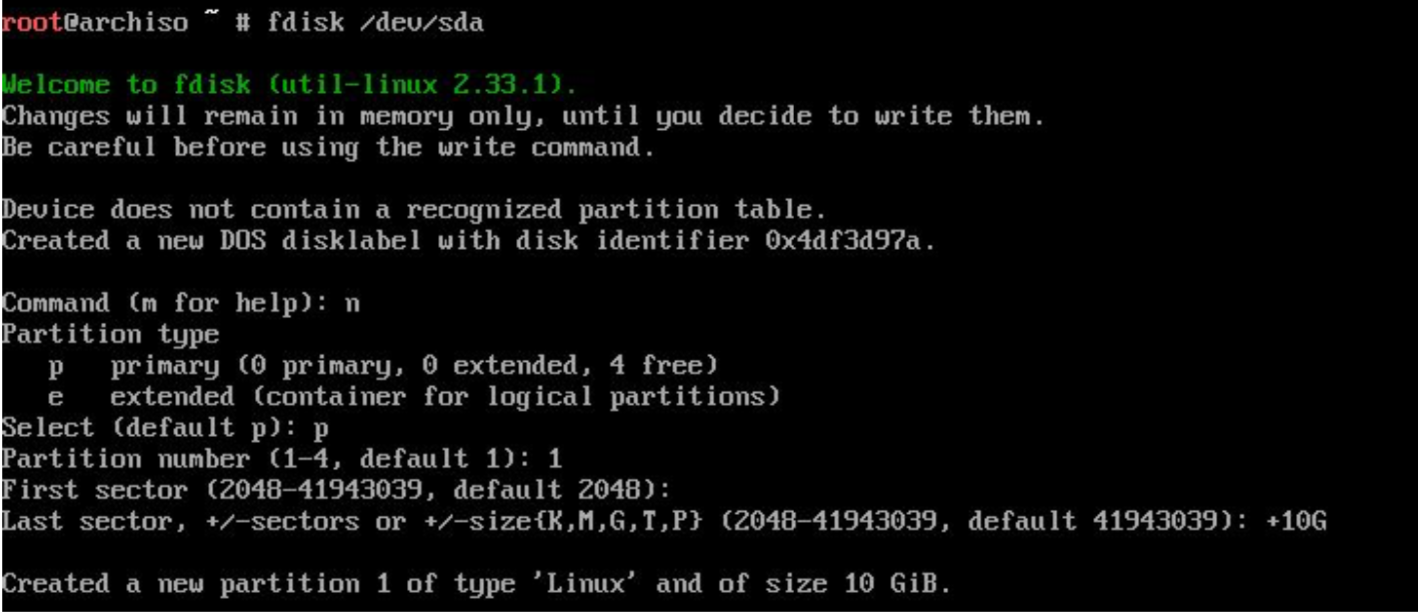
\includegraphics[width=0.8\textwidth]{img/3.png}
        \label{img:Imagen 3}
        \caption{fdisk /dev/sda: n,p,1,+10G}
\end{figure}
\begin{figure}[H]
        \centering
        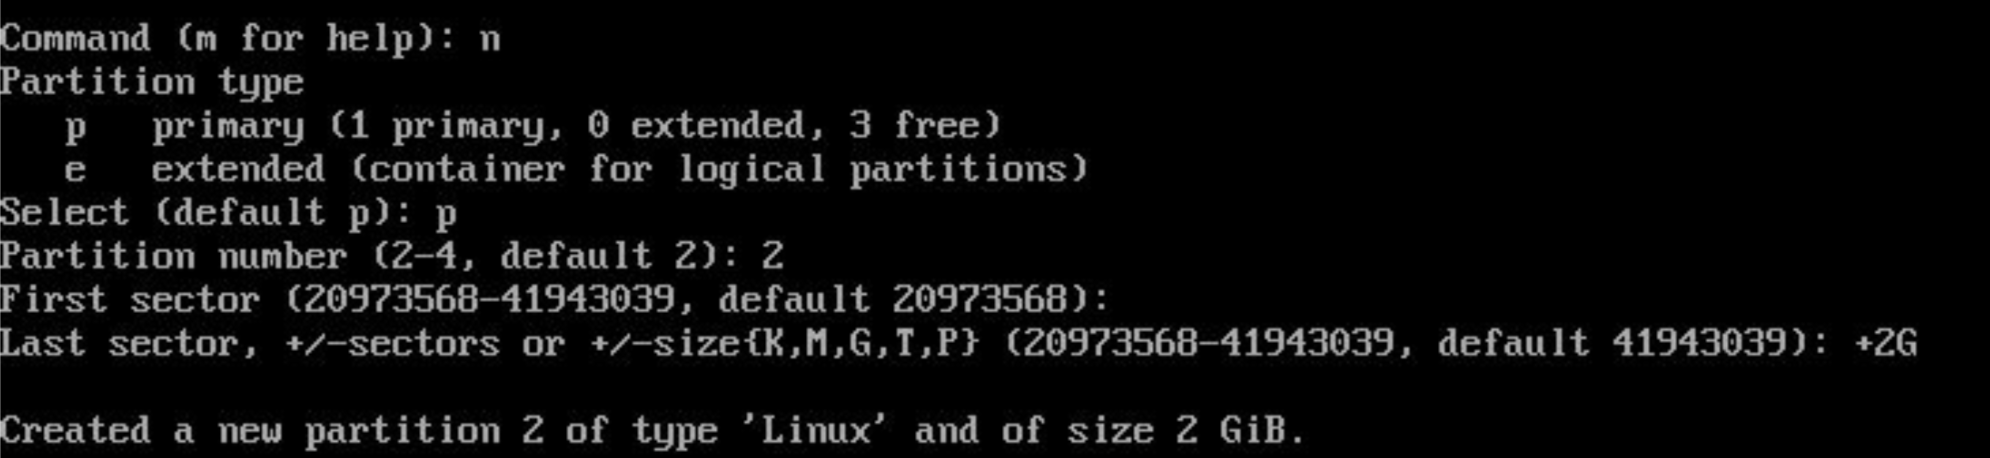
\includegraphics[width=0.8\textwidth]{img/4.png}
        \label{img:Imagen 4}
        \caption{fdisk /dev/sda: n,p,2,2}
\end{figure}
 \begin{figure}[H]
        \centering
        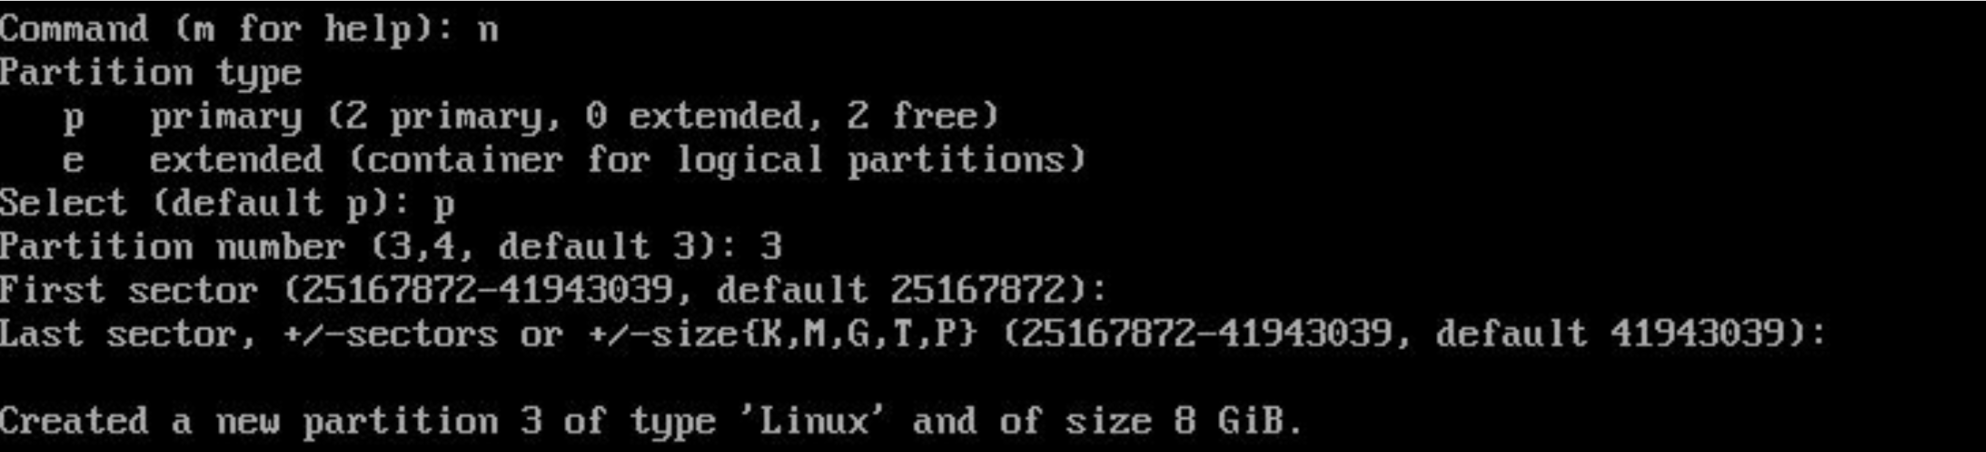
\includegraphics[width=0.8\textwidth]{img/5.png}
        \label{img:Imagen 4}
        \caption{fdisk /dev/sda: n,p,3,8}
\end{figure}
\begin{figure}[H]
        \centering
        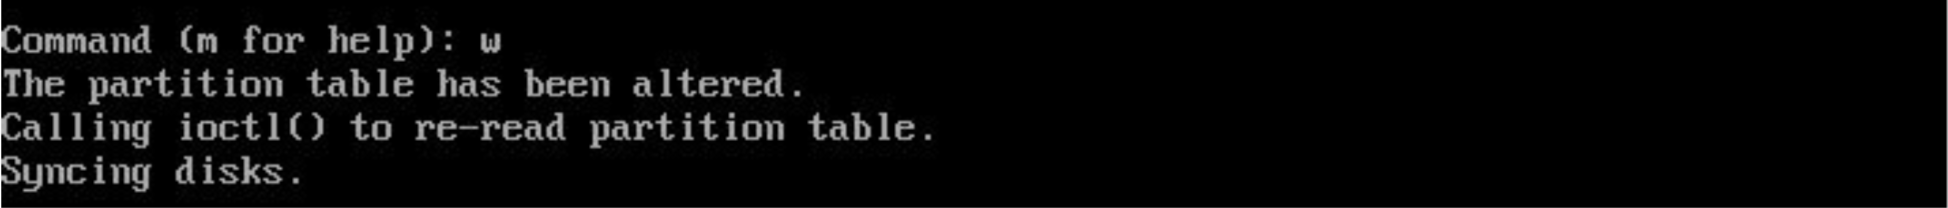
\includegraphics[width=0.8\textwidth]{img/6.png}
        \label{img:Imagen 4}
        \caption{Save changes}
\end{figure}
  Luego usamos el comando Linux MKFS, se  utiliza para dar formato a un dispositivo de almacenamiento de bloque con un determinado sistema de archivos, y lo usamos para / y /home (sda1 y sda3).
\begin{figure}[H]
        \centering
        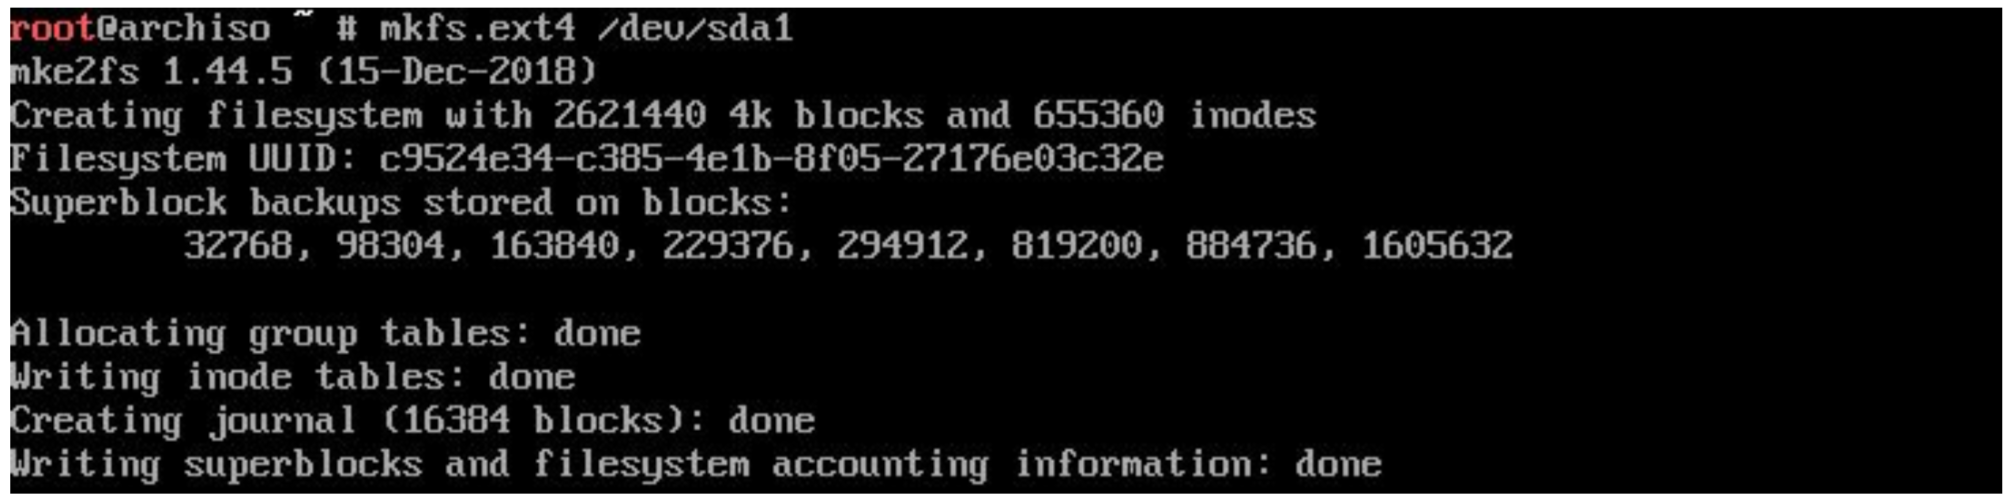
\includegraphics[width=0.8\textwidth]{img/7.png}
        \label{img:Imagen 4}
        \caption{/: mkfs.ext4 /dev/sda1}
\end{figure}
\begin{figure}[H]
        \centering
        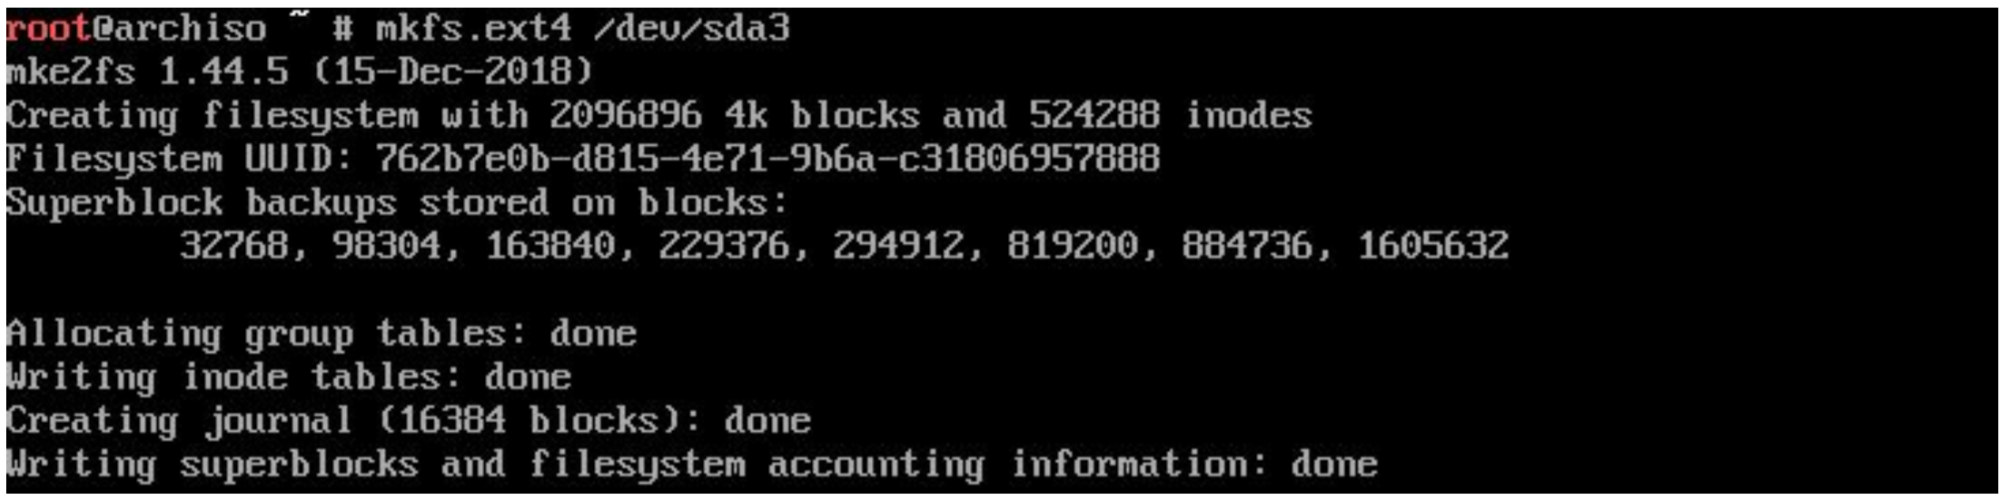
\includegraphics[width=0.8\textwidth]{img/8.png}
        \label{img:Imagen 4}
        \caption{/home: mkfs.ext4 /dev/sda3}
\end{figure} 
Usamos mkswap y swapon para crear espacio de intercambio.
\begin{figure}[H]
        \centering
        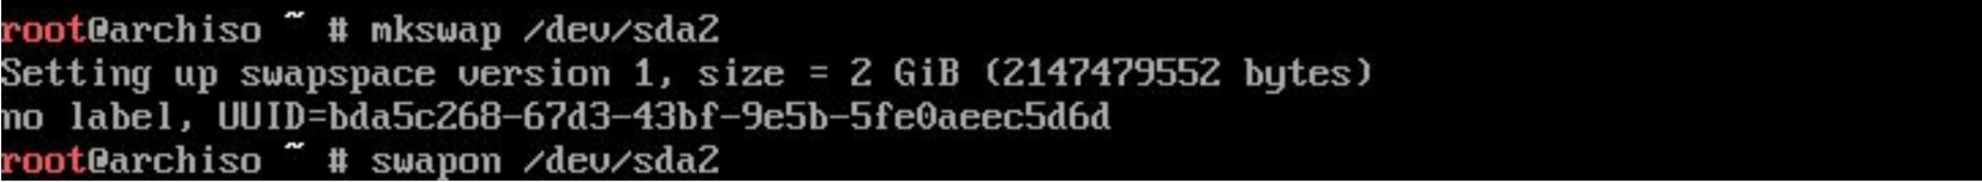
\includegraphics[width=0.8\textwidth]{img/9.png}
        \label{img:Imagen 4}
        \caption{swap: mkswap para sda2}
\end{figure}
Vamos a montar estos sistemas de archivos en la raíz y en home.
\begin{figure}[H]
        \centering
        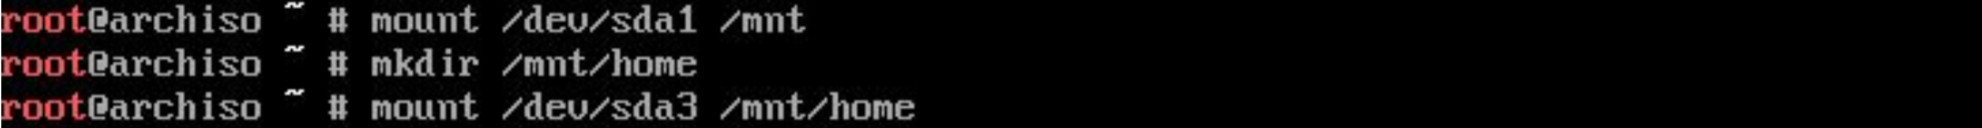
\includegraphics[width=0.8\textwidth]{img/10.png}
        \label{img:Imagen 4}
\end{figure}

Como hemos creado particiones y las hemos montado, instalemos el paquete base. Un paquete base contiene todo el paquete necesario para ejecutar un sistema, algunos de los cuales son el shell GNU BASH, herramienta de compresión de datos, utilidades del sistema de archivos, biblioteca C, herramientas de compresión, kernels y módulos Linux, paquetes de biblioteca, utilidades del sistema, utilidades de dispositivos USB , editor de texto vi, etc.
\begin{figure}[H]
        \centering
        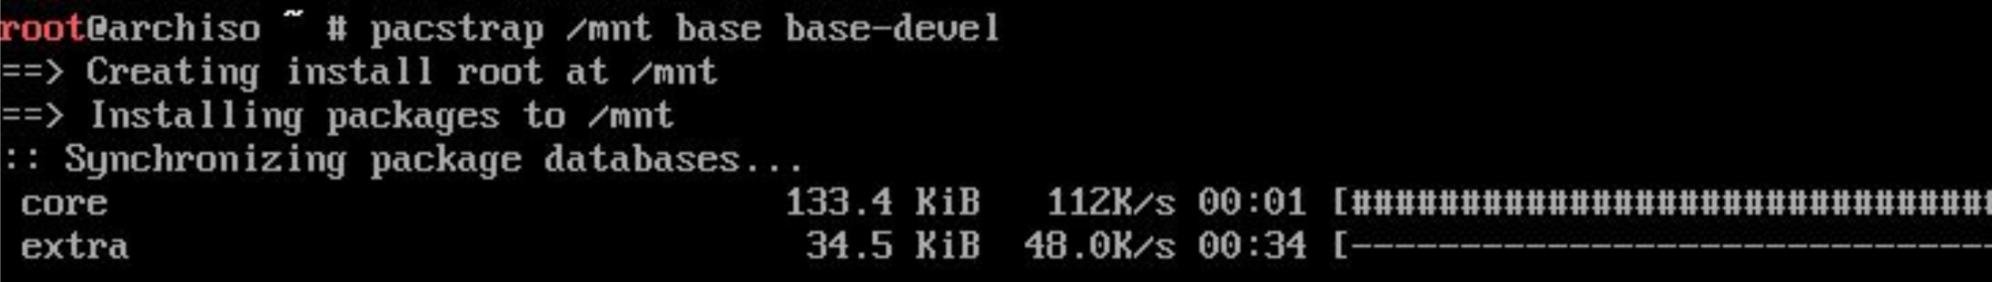
\includegraphics[width=0.8\textwidth]{img/11.png}
        \label{img:Imagen 4}
\end{figure}
\begin{figure}[H]
        \centering
        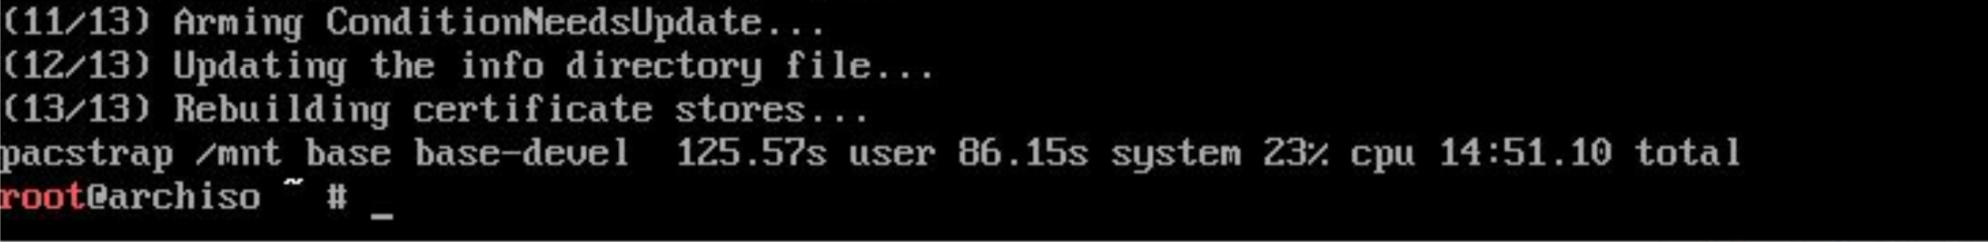
\includegraphics[width=0.8\textwidth]{img/12.png}
        \label{img:Imagen 4}
\end{figure}

Una vez instalado, debemos configurar el sistema generando un archivo \textit{fstab} para definir cómo las particiones de disco, dispositivos de bloque o sistemas de archivos remotos están montados en el sistema de archivos.
\begin{figure}[H]
        \centering
        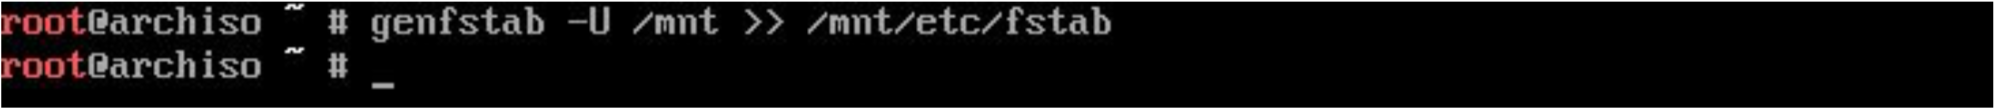
\includegraphics[width=0.8\textwidth]{img/13.png}
        \label{img:Imagen 4}
\end{figure}

Hasta el momento todo se ve como se muestra en la siguiente imagen, lo que ahora tenemos que hacer es montar dispositivos y particiones para su uso por el sistema operativo. Montar es hacer que el sistema operativo proyecte el contenido de ese dispositivo o partición en un enlace lógico (un directorio). 
\begin{figure}[H]
        \centering
        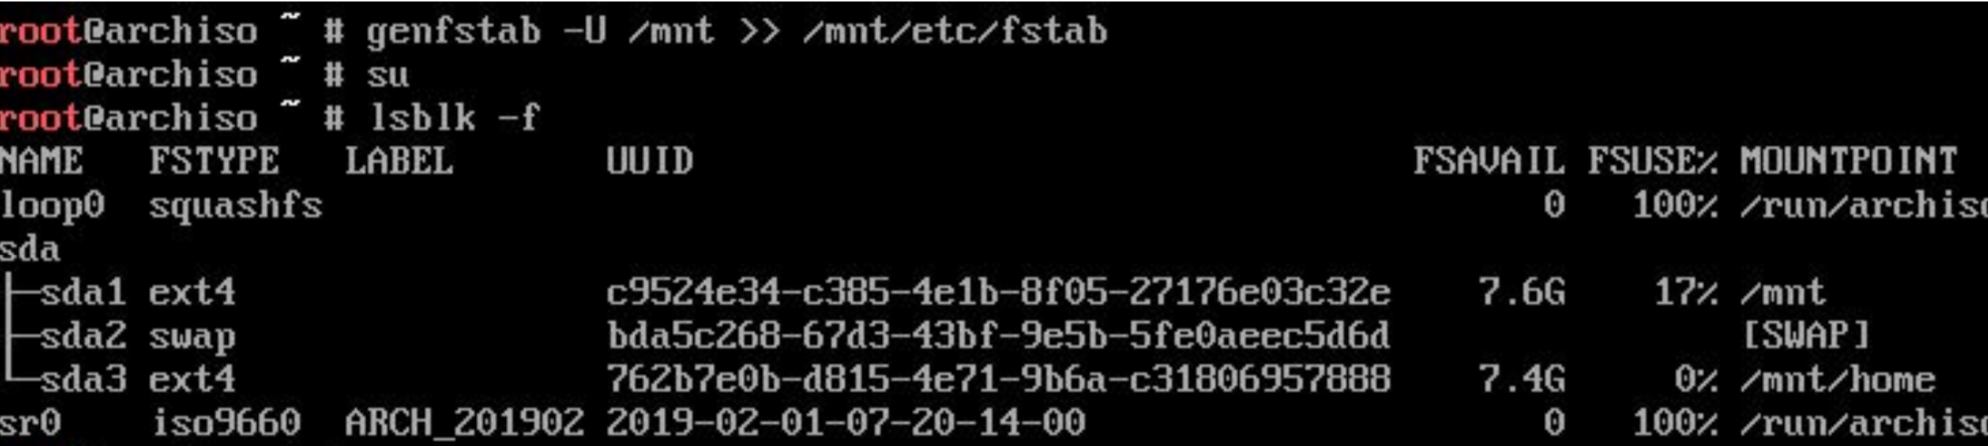
\includegraphics[width=0.8\textwidth]{img/14.png}
        \label{img:Imagen 4}
        \caption{listando las particiones}
\end{figure}

\begin{figure}[H]
        \centering
        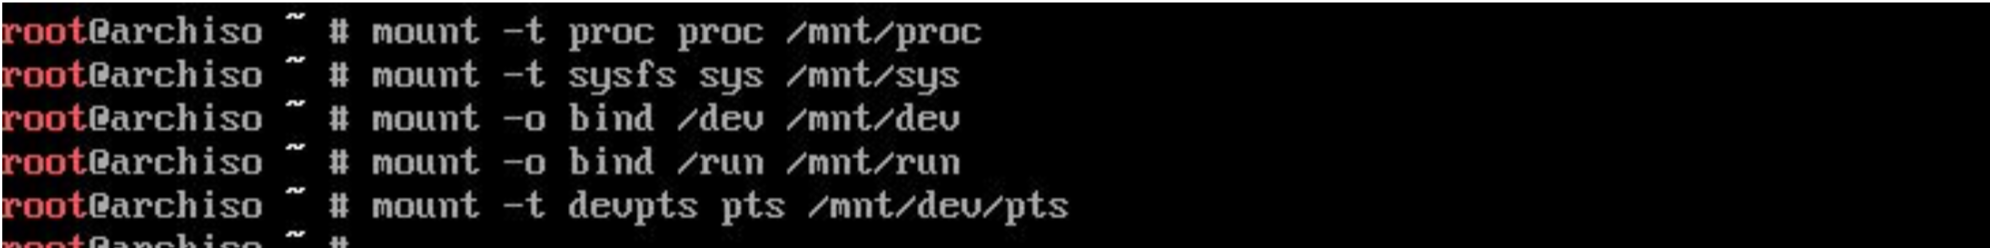
\includegraphics[width=0.8\textwidth]{img/15.png}
        \label{img:Imagen 4}
\end{figure}
Ahora tenemos que configurar el servidor dns.
\begin{figure}[H]
        \centering
        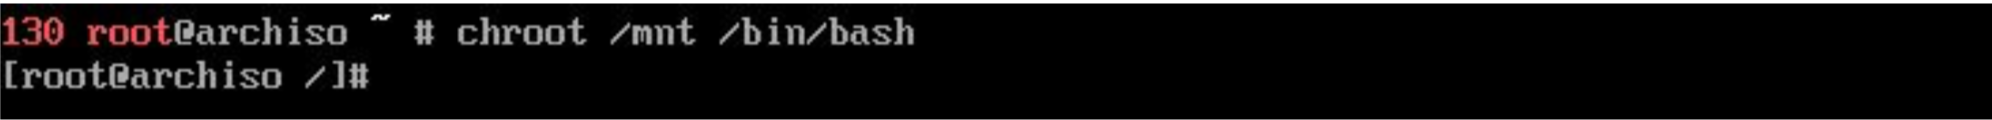
\includegraphics[width=0.8\textwidth]{img/17.png}
        \label{img:Imagen 4}
\end{figure}
Luego cambiamos el root al nuevo sistema, esto permite cambiar el directorio raíz para el proceso en ejecución actual y el proceso hijo.
\begin{figure}[H]
        \centering
        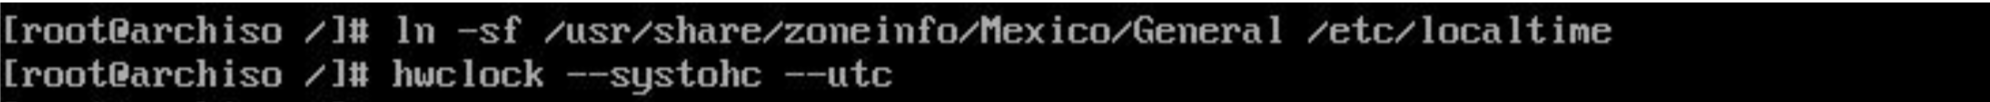
\includegraphics[width=0.8\textwidth]{img/18.png}
        \label{img:Imagen 4}
\end{figure}

Ahora hay que configurar de la zona horaria como en cualquier dispositivo Linux.
\begin{figure}[H]
        \centering
        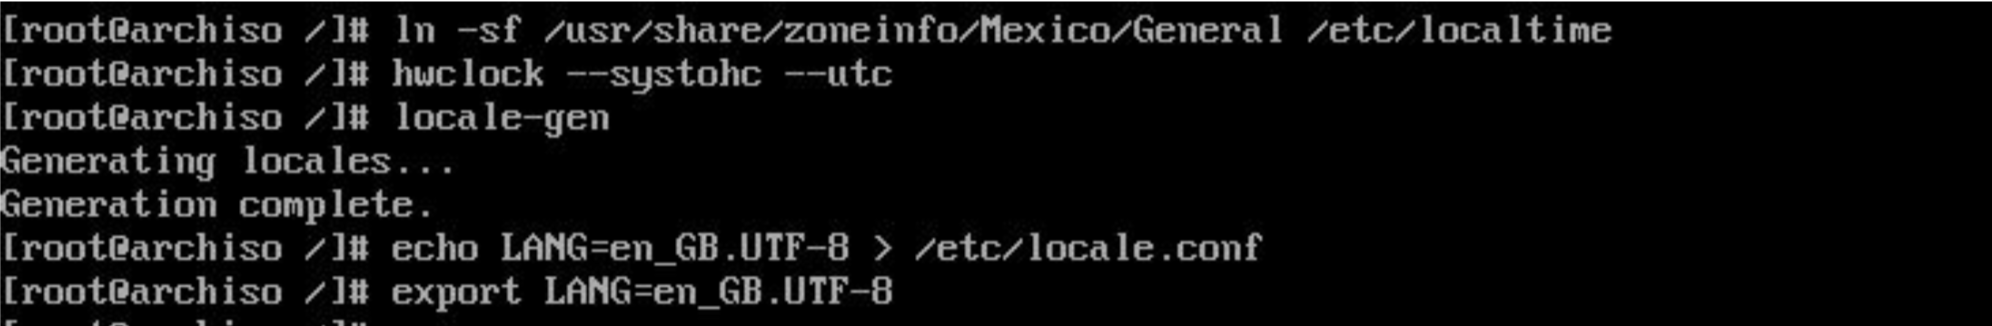
\includegraphics[width=0.8\textwidth]{img/19.png}
        \label{img:Imagen 4}
\end{figure}

Después de configurar la zona horaria, hay que configurar Locale. El archivo /etc/locale.gen contiene todas las configuraciones locales y el idioma del sistema en un formato comentado. 

\begin{figure}[H]
        \centering
        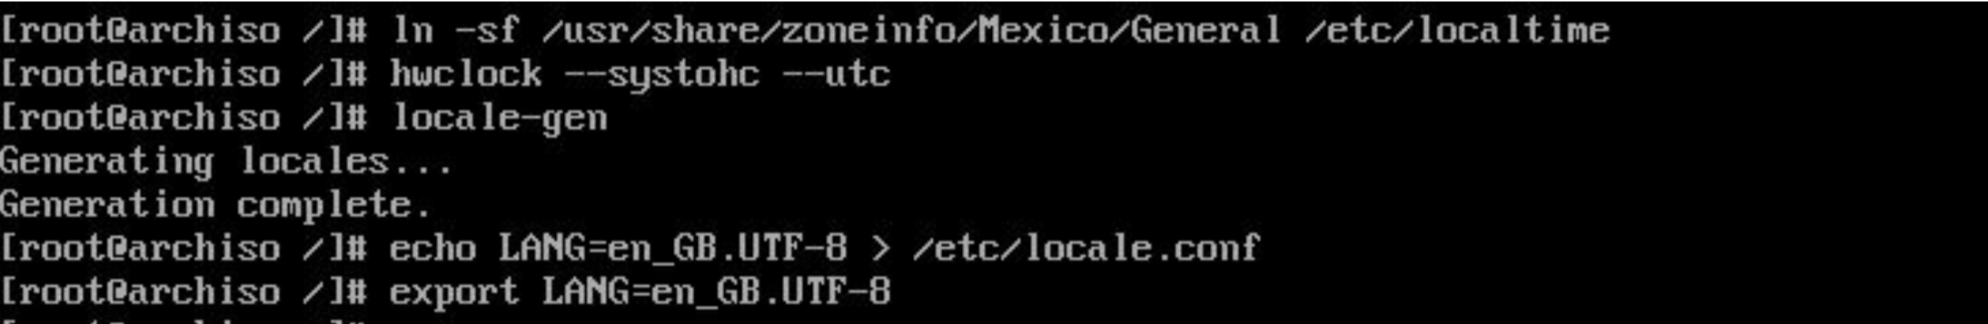
\includegraphics[width=0.8\textwidth]{img/20.png}
        \label{img:Imagen 4}
\end{figure}
Y tenemos que configurar del nombre de host.
\begin{figure}[H]
        \centering
        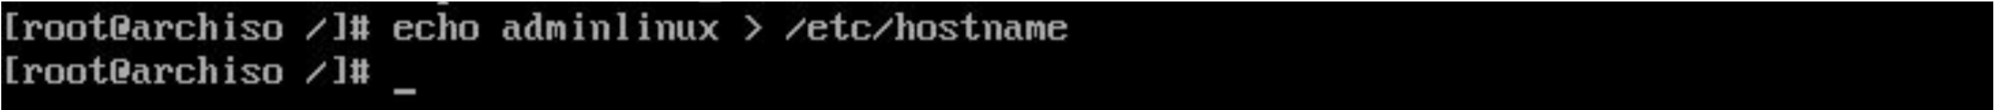
\includegraphics[width=0.8\textwidth]{img/21.png}
        \label{img:Imagen 4}
\end{figure}
Para instalar un gestor de arranque hicimos los siguientes pasos.
\begin{figure}[H]
        \centering
        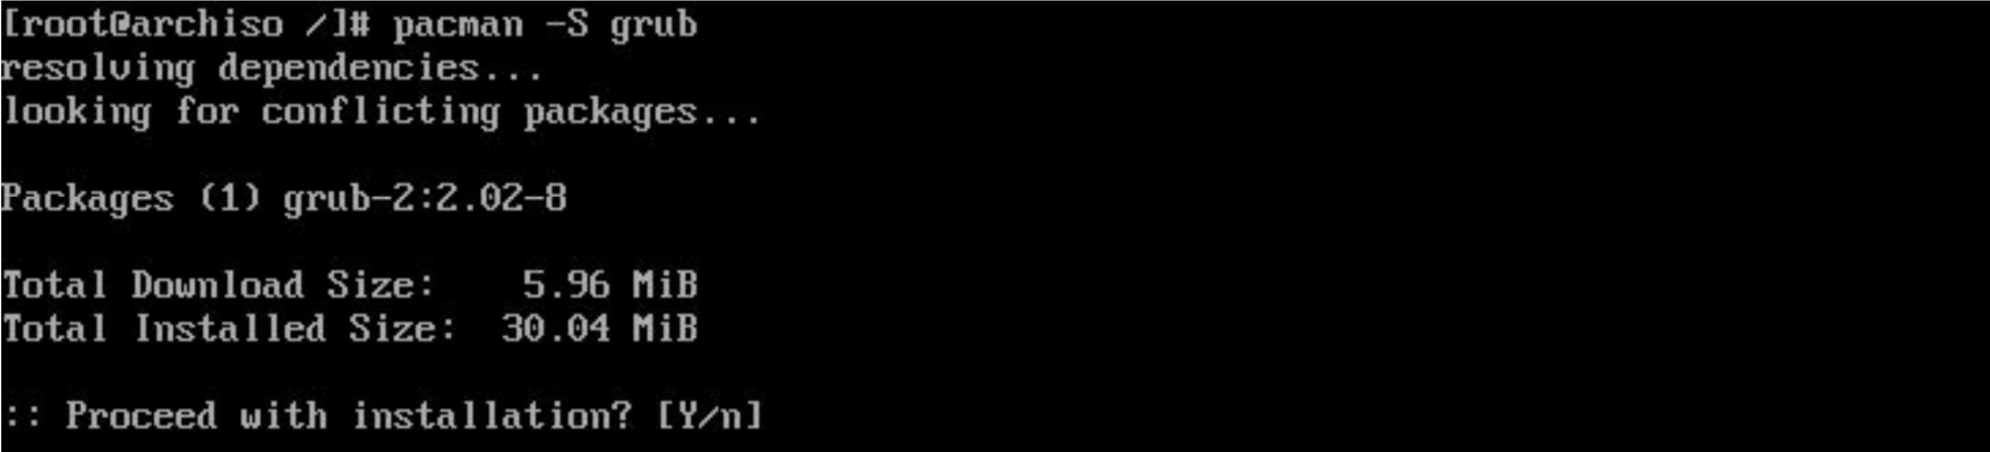
\includegraphics[width=0.8\textwidth]{img/22.png}
        \label{img:Imagen 4}
\end{figure}
\begin{figure}[H]
        \centering
        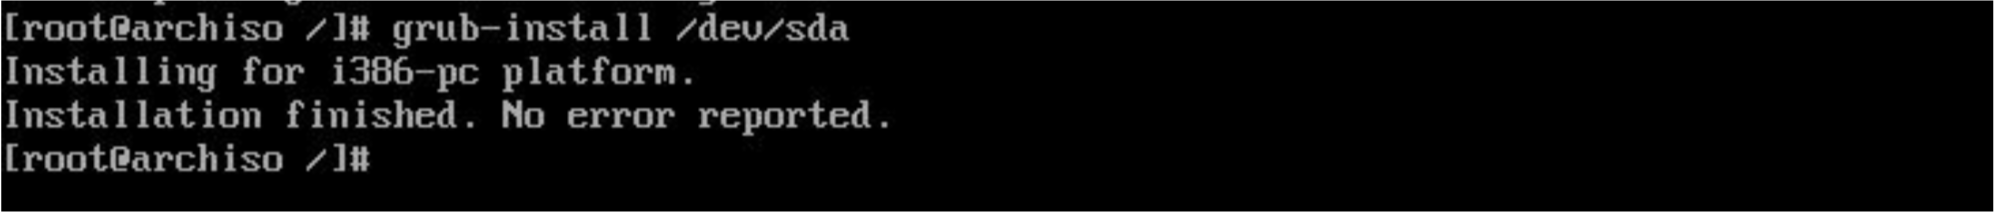
\includegraphics[width=0.8\textwidth]{img/23.png}
        \label{img:Imagen 4}
\end{figure}
\begin{figure}[H]
        \centering
        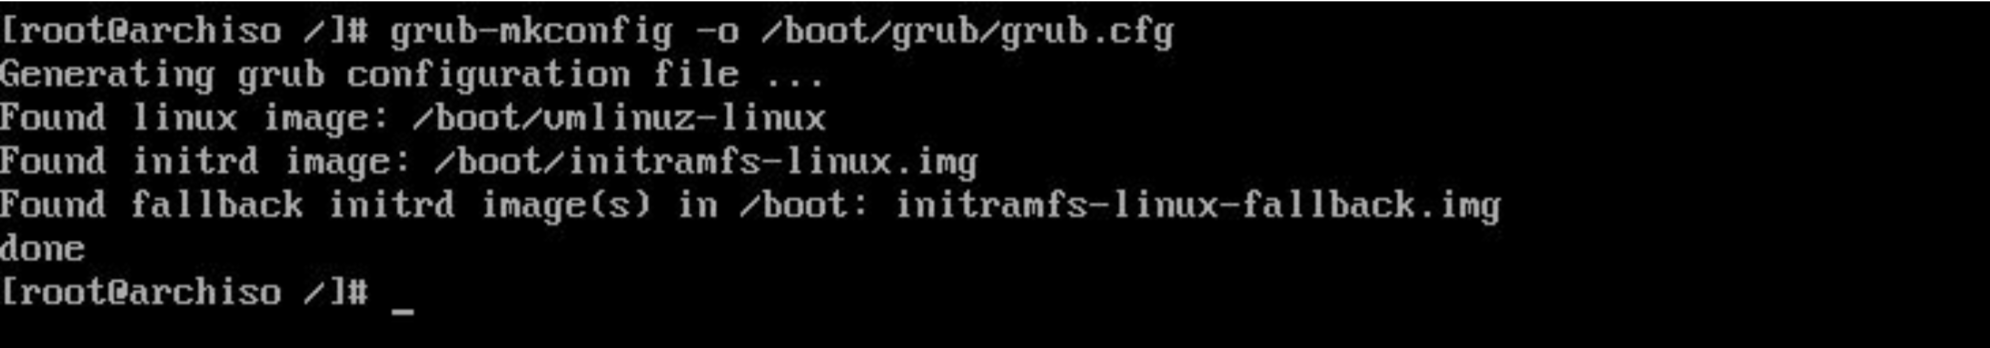
\includegraphics[width=0.8\textwidth]{img/24.png}
        \label{img:Imagen 4}
\end{figure}

Y para crear la contraseña root usamos el comando \textit{passwd}.

\begin{figure}[H]
        \centering
        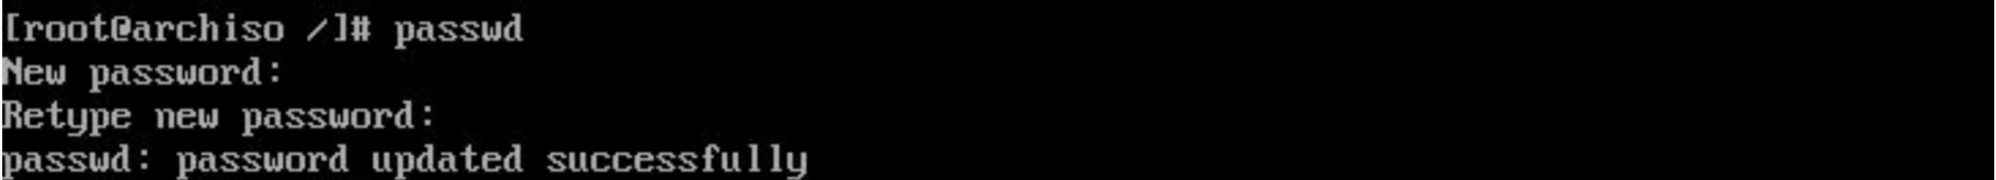
\includegraphics[width=0.8\textwidth]{img/25.png}
        \label{img:Imagen 4}
\end{figure}
Una vez hecho, actualizamos nuestro nuevo sistema. 
\begin{figure}[H]
        \centering
        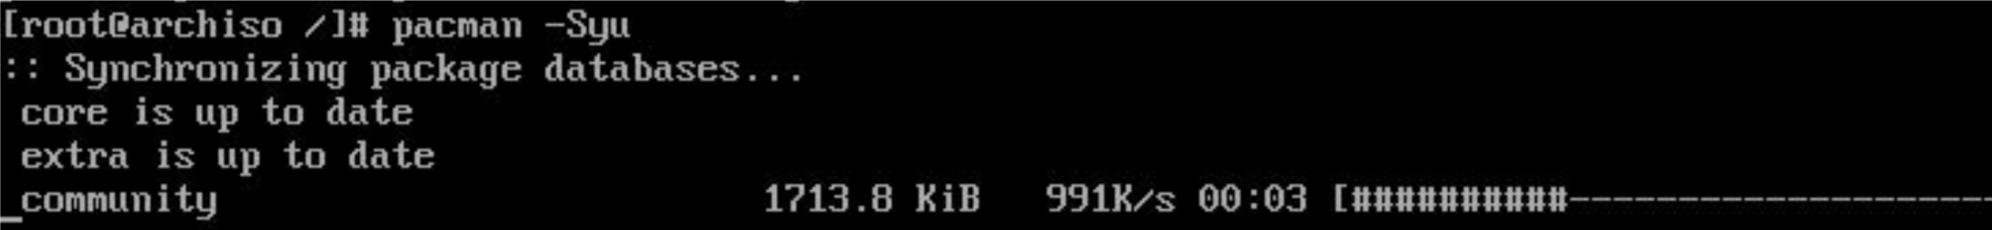
\includegraphics[width=0.8\textwidth]{img/26.png}
        \label{img:Imagen 4}
\end{figure}
\begin{figure}[H]
        \centering
        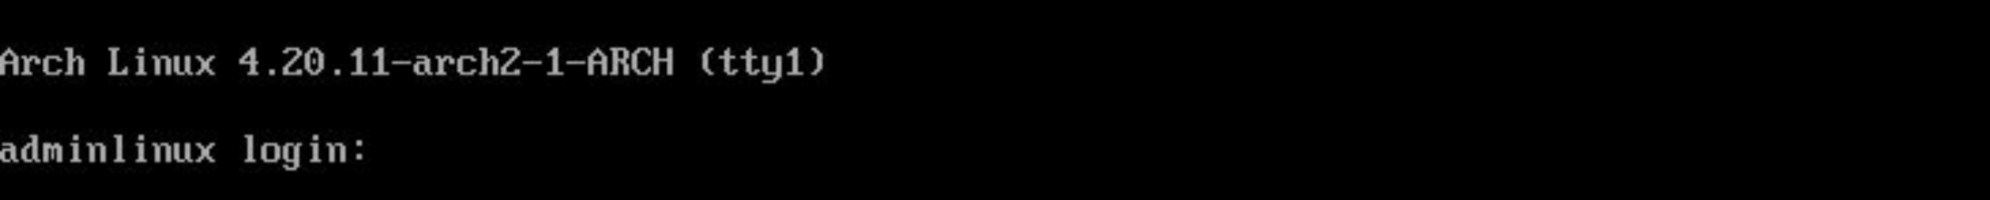
\includegraphics[width=0.8\textwidth]{img/27.png}
        \label{img:Imagen 4}
\end{figure}
\begin{figure}[H]
        \centering
        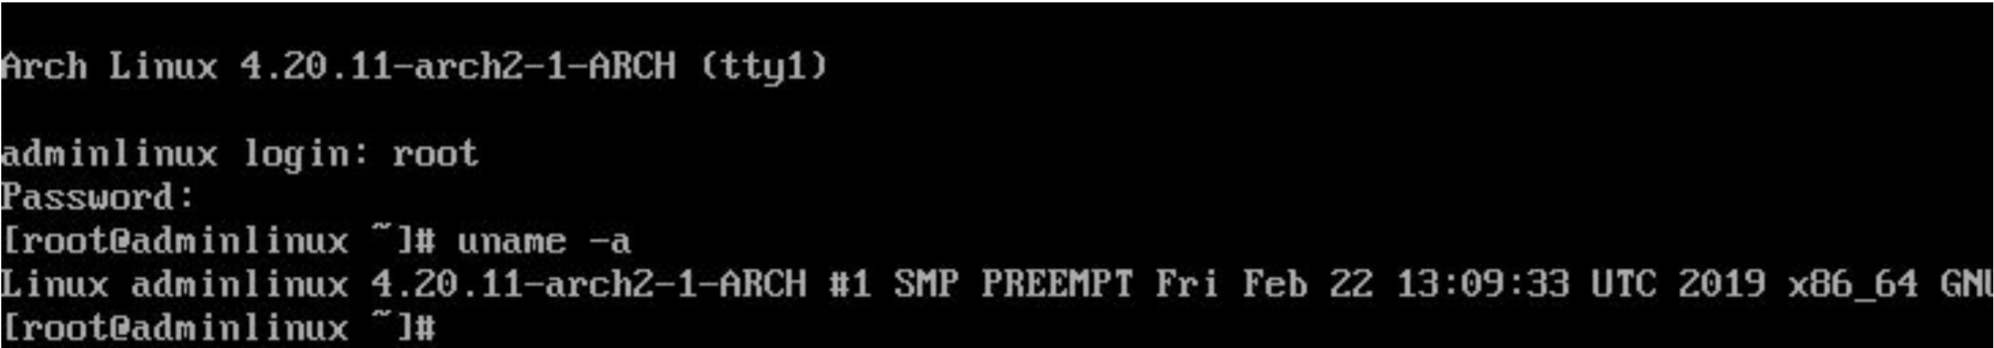
\includegraphics[width=0.8\textwidth]{img/28.png}
        \label{img:Imagen 4}
\end{figure}

\subsection{GNOME}

Hemos instalado hasta el momento con éxito una línea de comando mínima Arch Linux y ahora veremos cómo configurar un entorno de escritorio o una Interfaz gráfica de usuario para Arch Linux llamado GNOME.

Necesitamos una serie de prerequisitos para intalar GNOME, o cualquier entorno de escritorio, primero debemos configurar la red.
\begin{figure}[H]
        \centering
        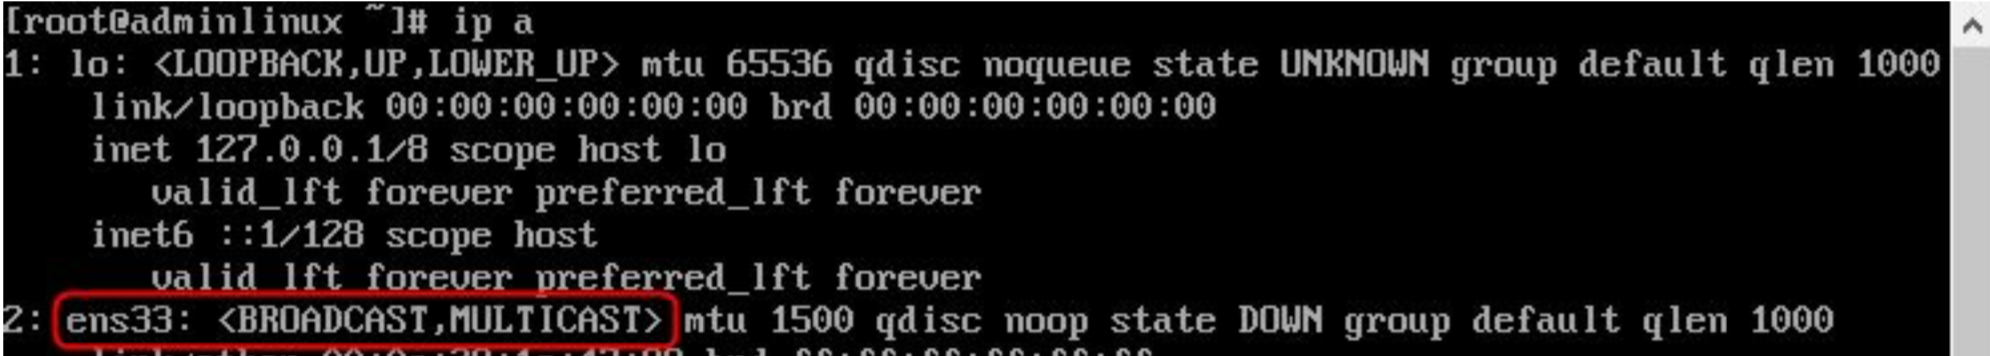
\includegraphics[width=0.8\textwidth]{img/29.png}
        \label{img:Imagen 4}
\end{figure}
Y tenemos que agregae las siguientes entradas en el archivo \textit{vi /etc/systemd/network/ens33.network}.
\begin{figure}[H]
        \centering
        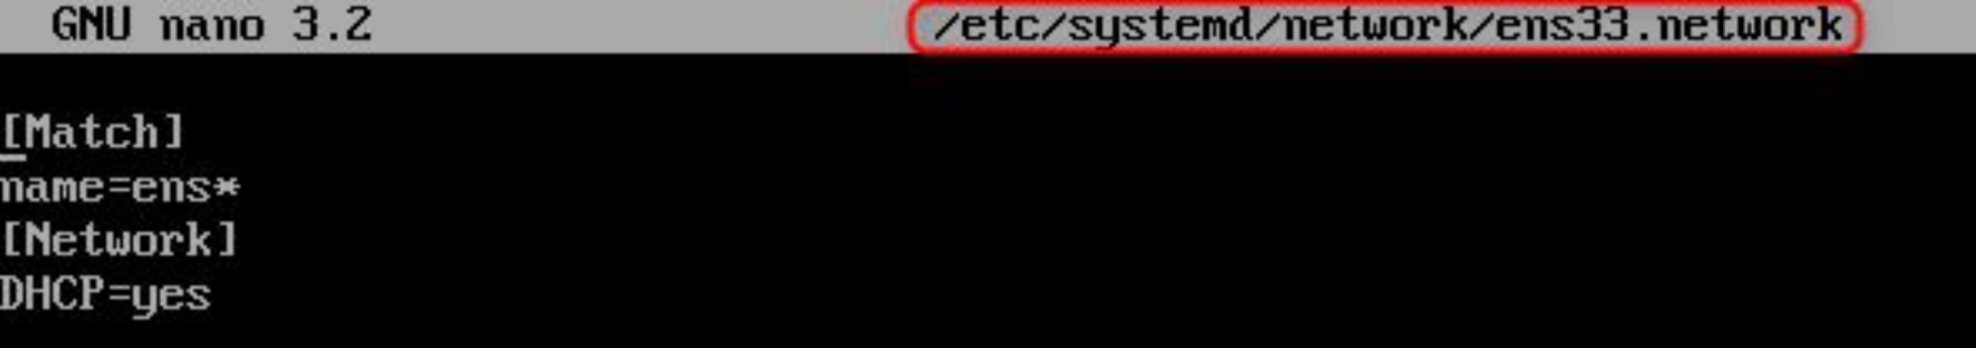
\includegraphics[width=0.8\textwidth]{img/30.png}
        \label{img:Imagen 4}
\end{figure}

Finalmente guardamos y salimos, reiniciamos la red con systemd para que los cambios se reflejen.
\begin{figure}[H]
        \centering
        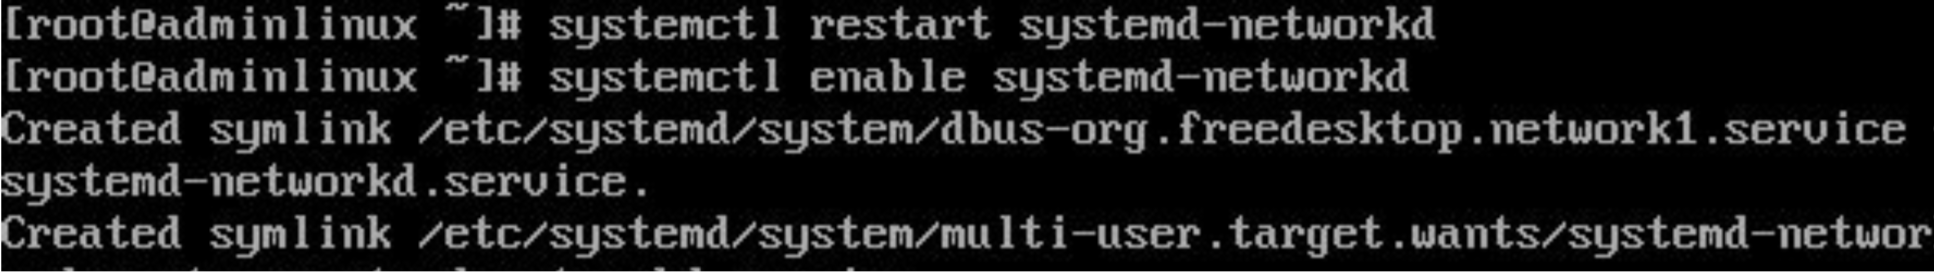
\includegraphics[width=0.8\textwidth]{img/31.png}
        \label{img:Imagen 4}
\end{figure}
Y agregamos dos entradas siguientes en \textit{/etc/resolv.conf}.
\begin{figure}[H]
        \centering
        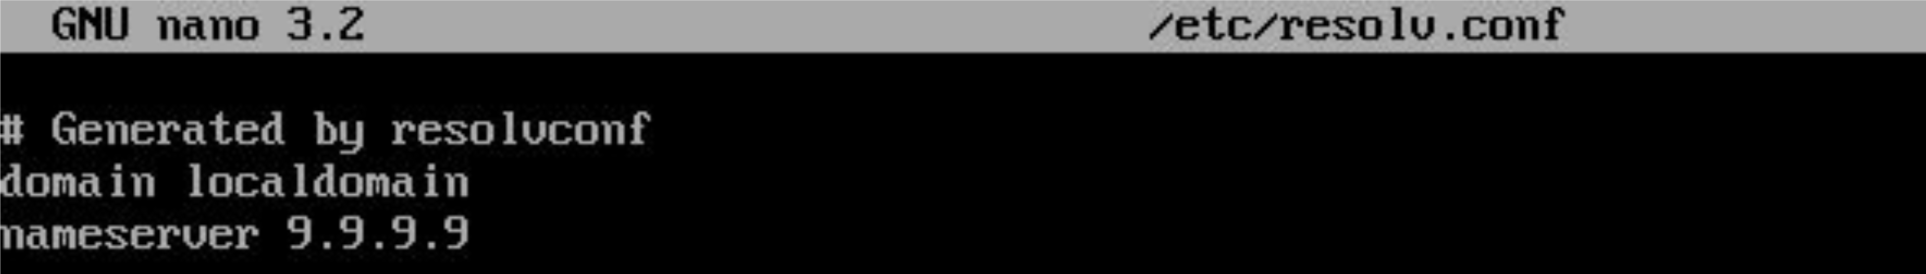
\includegraphics[width=0.8\textwidth]{img/32.png}
        \label{img:Imagen 4}
\end{figure}
El siguiente paso es instalar el entorno X e Xorg como servidor de visualización. Xorg es básicamente el sistema de ventanas X utilizado en Linux. Es la base del entorno gráfico para tu computadora. 

\begin{figure}[H]
        \centering
        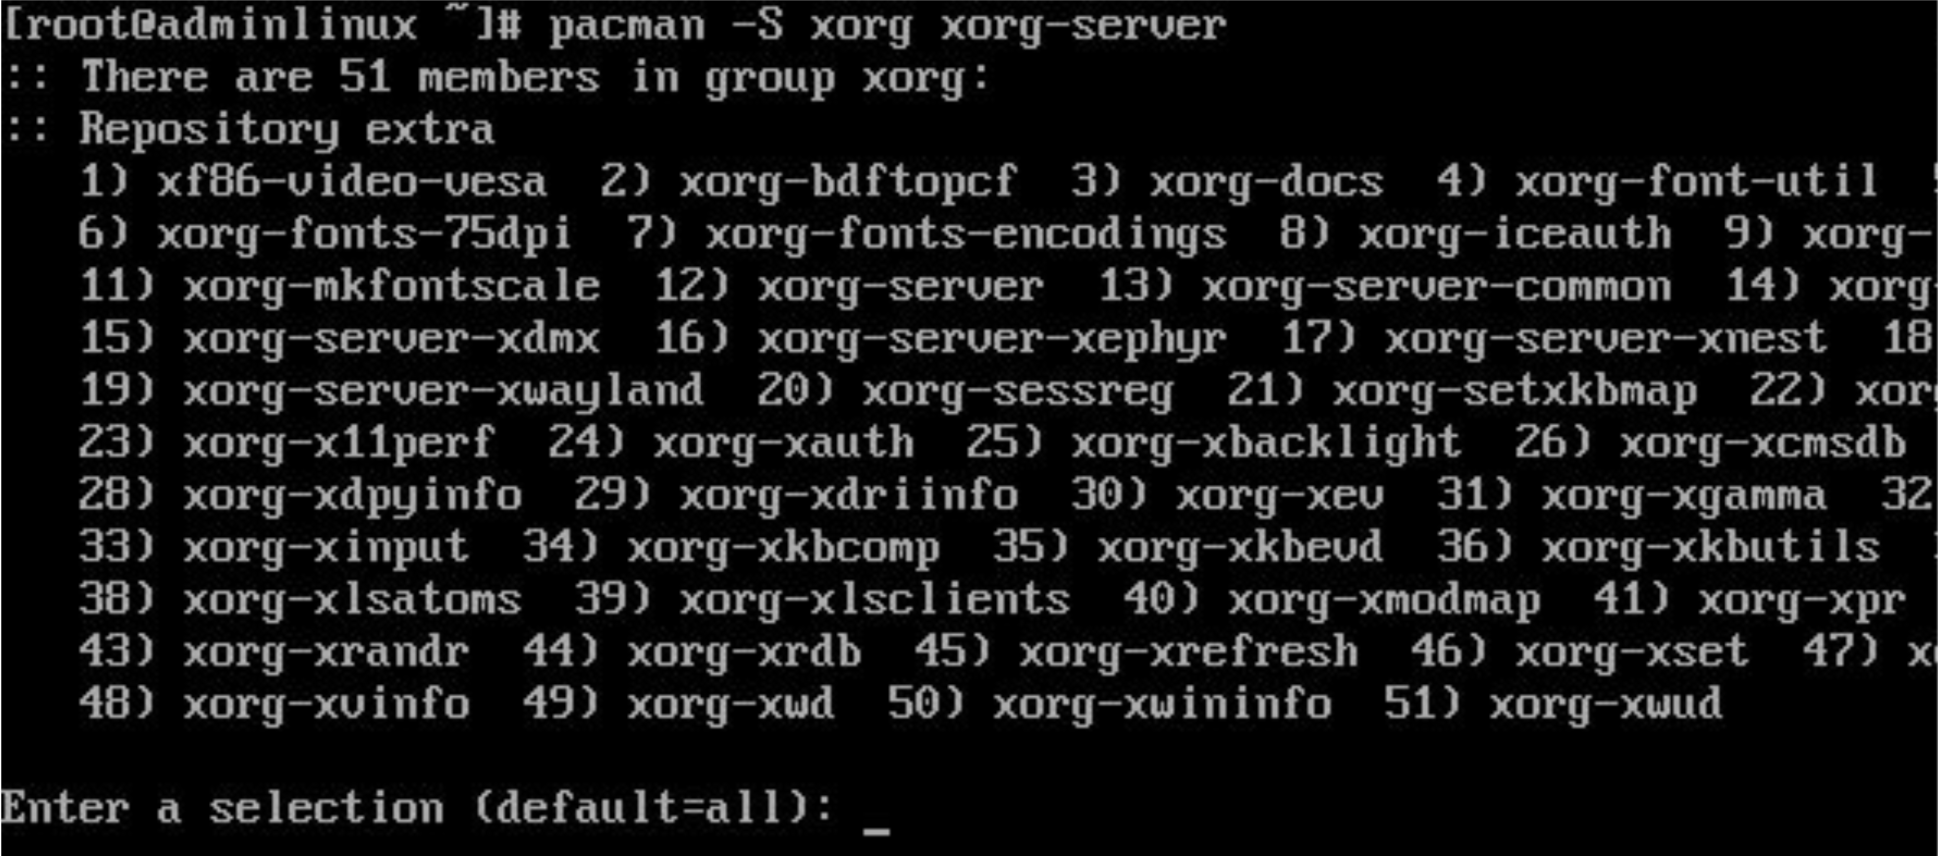
\includegraphics[width=0.8\textwidth]{img/33.png}
        \label{img:Imagen 4}
\end{figure}


GNOME contiene el escritorio base de GNOME. gnome-extra contiene aplicaciones de GNOME, administrador de archivos, administrador de discos, editores de texto y más. El último paso incluye habilitar el administrador de visualización GDM para Arch usando el comando \textit{systemctl start gdm.service}.


\begin{figure}[H]
        \centering
        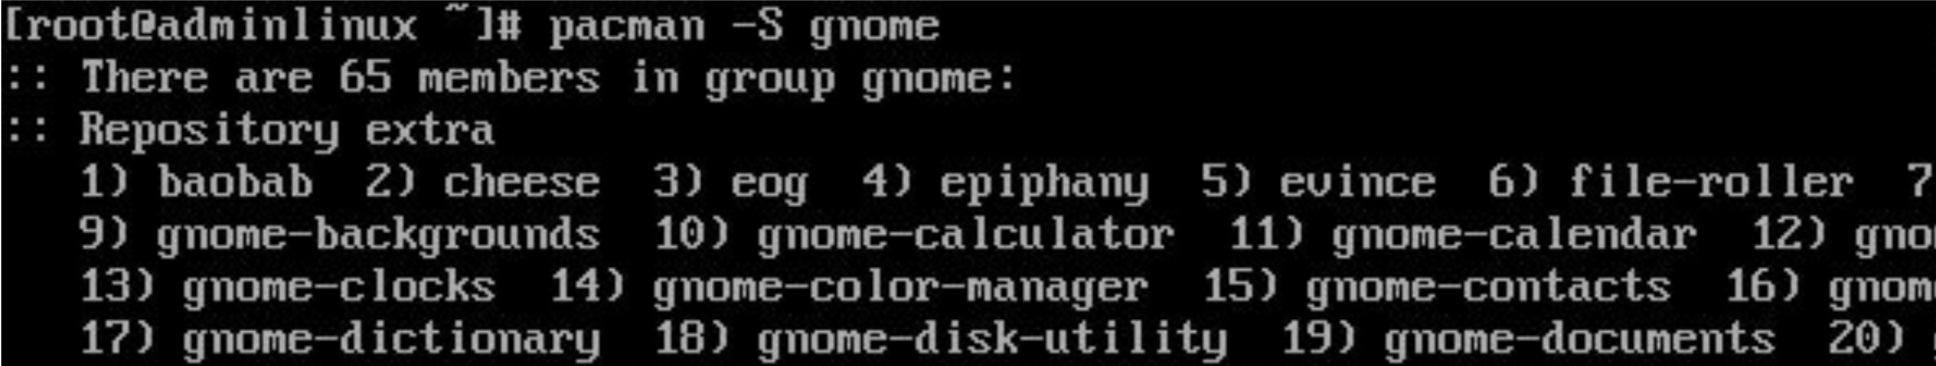
\includegraphics[width=0.8\textwidth]{img/34.png}
        \label{img:Imagen 4}
\end{figure}


\begin{figure}[H]
        \centering
        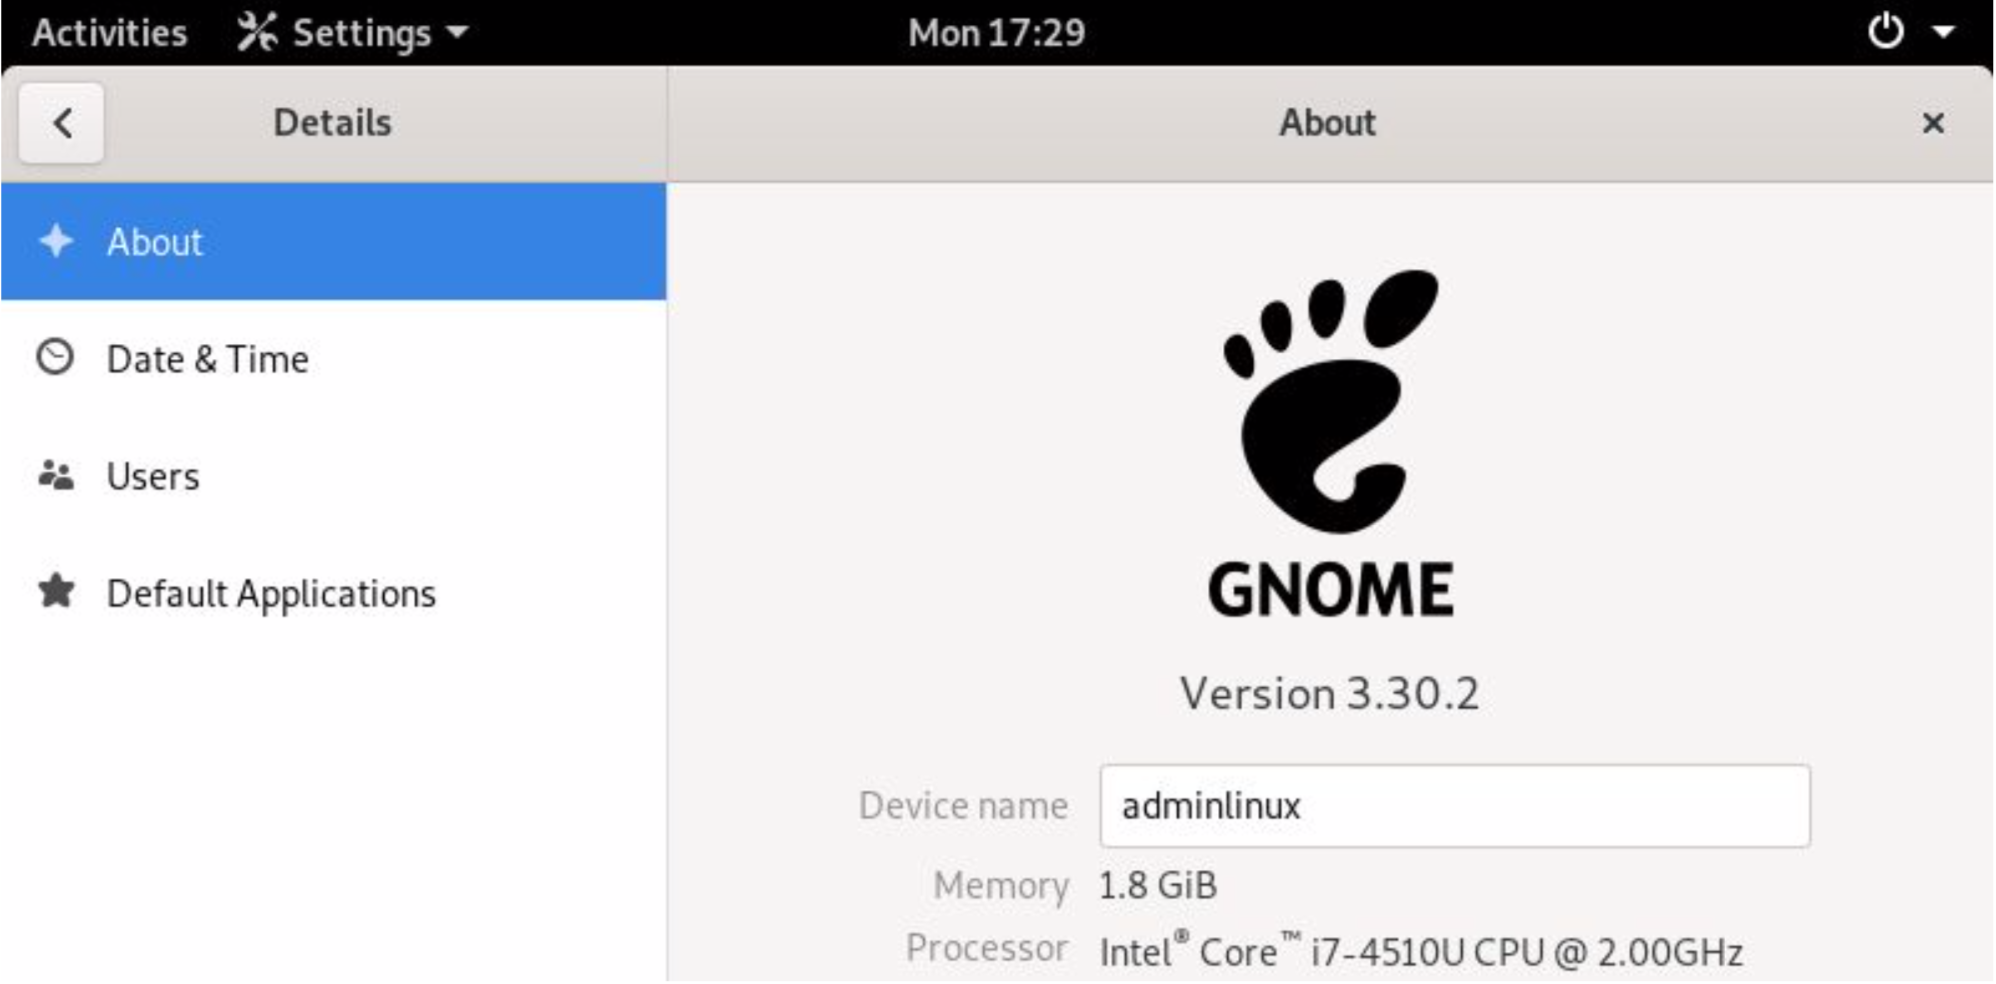
\includegraphics[width=0.8\textwidth]{img/35.png}
        \label{img:Imagen 4}
\end{figure}

\section{Referencias}
\begin{thebibliography}{}
\bibitem{install arch} 
\url{https://maslinux.es/como-instalar-arch-linux-paso-a-paso/}
\bibitem{install arch2} 
\url{https://wiki.archlinux.org/index.php/Installation_guide_(Español)}
\bibitem{xor} 
\url{https://ubuntuforums.org/showthread.php?t=955672}
\bibitem{mkfs} 
\url{https://www.servidoresadmin.com/comando-linux-mkfs/}
\bibitem{dns} 
\url{https://serverfault.com/questions/905903/networkmanager-dnsmasq-ignore-auto-dns-settings}
\end{thebibliography}

\end{document}


